\documentclass[12pt]{article}

\usepackage{sbc-template}

\usepackage{graphicx,url}

\usepackage[brazil]{babel}   
%\usepackage[latin1]{inputenc}  
\usepackage[utf8]{inputenc}  
% UTF-8 encoding is recommended by ShareLaTex
\usepackage{placeins}
\usepackage[section]{placeins}
\usepackage[subsection]{placeins}
     
\sloppy

\title{Implementação de Banco de Dados em Diário de Classe\\ com MySQL E PyQT}

\author{José Victor Viriato, Gabriel Haddad }


\address{Departamento de Informática -- Universidade Federal de Santa Maria
  (UFSM)\\
  \email{\{jvviriato,ghvieira\}@inf.ufsm.br}
}

\begin{document} 

\maketitle

\begin{abstract}
  Tis paper exposes the work of UFSM's Computer Science students on the development of a database for an univerr'sity that needs to computerize its students frequency control. The most important informations, such as functions, triggers, tools, tables and views will be exposend and explained during the paper.
\end{abstract}
     
\begin{resumo} 
  Este artigo expõe o trabalho de alunos do Curso de Ciência da Computação da UFSM no desenvolvimento de um banco de dados para uma universidade que necessita informatizar no controle de frequência de seus alunos. As informações mais importantes, como funções, triggers, ferramentas, tabelas e views serão expostas e explicadas durante o artigo.
\end{resumo}


\section{Introdução}

O presente artigo apresenta um projeto desenvolvido pelos alunos Gabriel Haddad e José Viriato da Universidade Federal de Santa Maria, docentes do curso de Ciência da Computação. O texto relata em detalhes a ideia basica do projeto, bem como as ferramentas utilizadas ao longo deste, as funções, tabelas, trigger, views e diagrama desenvolvidos. 


\section{Problema Inicial} \label{sec:probinic}


O objetivo final do artigo era de conseguir solidificar a ideia de um banco de dados para uma universidade que deseja informatizar seu diário de frequência dos alunos. O banco teria como tabelas: Alunos, Disciplinas, Cursos, Turmas, Professores e Frequência. Desse modo, as tabelas foram criadas e bem como, algumas, interligadas.



\section{Ferramentas Utilizadas}\label{sec:ferrusd}


Durante a realização do presente trabalho, diversas ferramentas foram utilizadas para completá-lo. Inicialmente a plataforma GitHub\cite{jviriato:2017} foi de extrema necessidade para a dupla, na qual frequentemente atualizava-se os arquivos do trabalho bem como acompanhava seu progresso. Para a Figura 1 - Diagrama de Classe do Banco de Dados - foi utilizada a ferramenta Astah\cite{astah}. MySQL, MySQL Workbench\cite{mysqlworkbench}, Python3\cite{python3} juntamente com PyCharm\cite{pycharm} e PyMySQL surgiram a seguir, como itens fundamentais para o projeto. Na sequência, para a construção das interfaces das tabelas, o QtDesigner\cite{qt} juntamente com o PyQt foram necessários. Por fim, para a construção do presente artigo, a ferramenta LaTeX\cite{latex} foi utilizada.



\section{Implementação do Banco de Dados}\label{sec:impbd}

\subsection{Diagrama de Classe}

O Diagrama de Classe abaixo (Figura~\ref{fig:exampleFig1}) ilustra todas as tabelas presentes no banco de dados que o presente artigo descreve, bem como suas chaves e chaves estrangeiras.
\begin{figure}[ht]
\centering
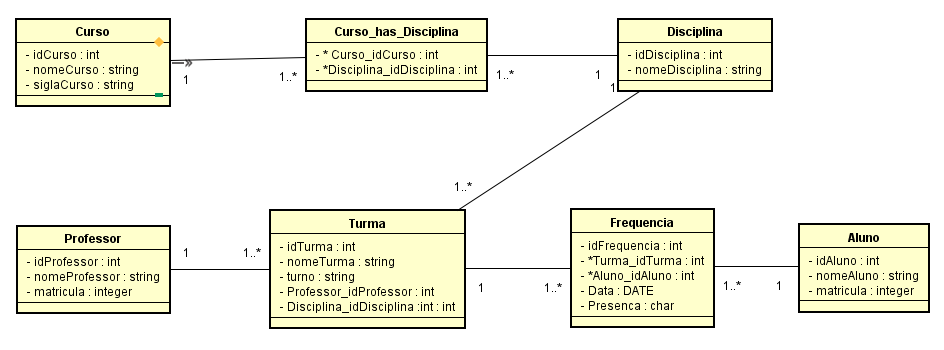
\includegraphics[width=1\textwidth]{Pic01.png}
\caption{Diagrama de Classe}
\label{fig:exampleFig1}
\end{figure}
\clearpage 

\subsection{Tabelas}

\begin{figure}[!htb]
\centering
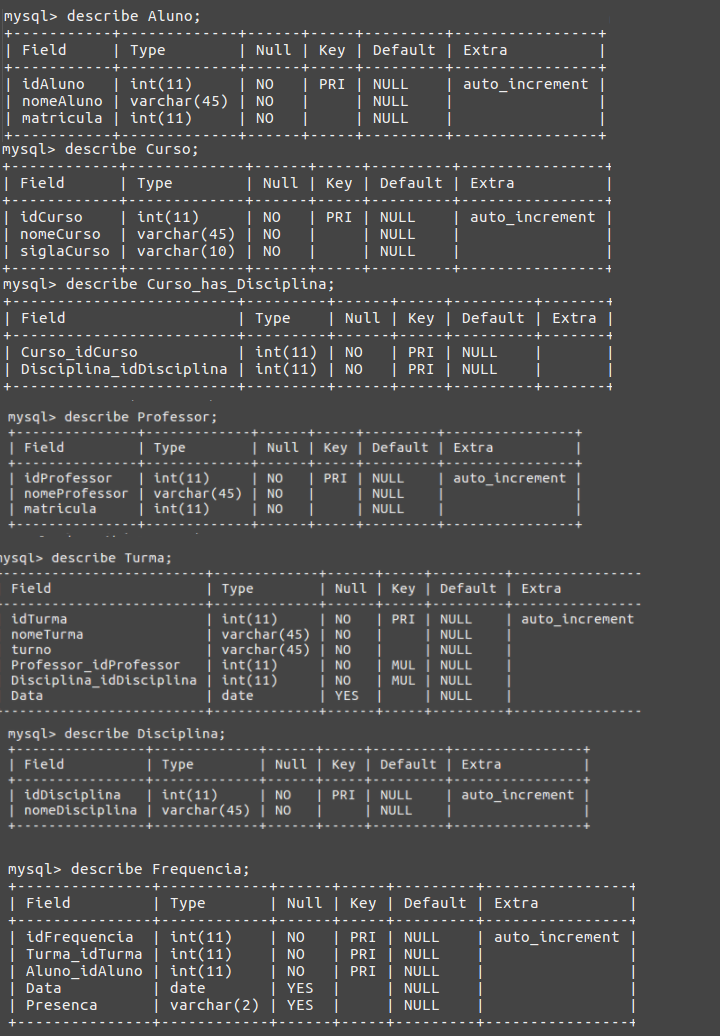
\includegraphics[width=1\textwidth]{Tabelas_Final.png}
\caption{Tabelas usadas no Banco de Dados}
\label{fig:exampleFig3}
\end{figure}
\clearpage 
\subsection{Views}
\begin{figure}[!htb]
\centering
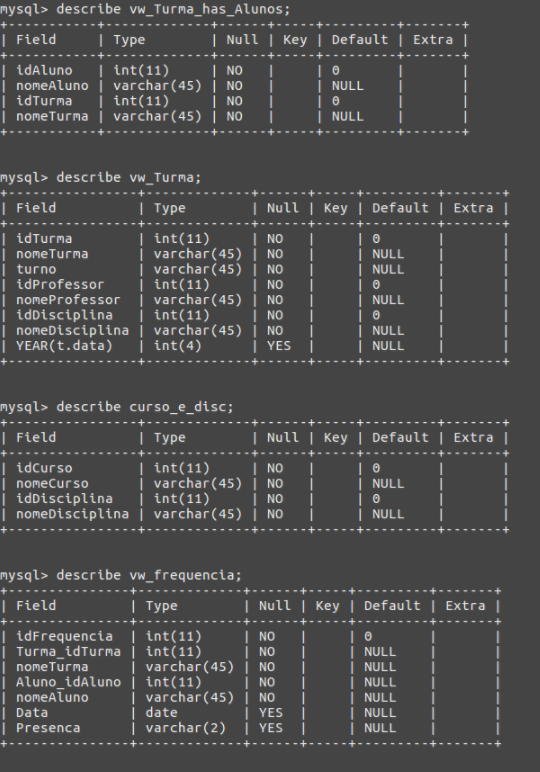
\includegraphics[width=1\textwidth]{views_Final.png}
\caption{Views usadas no Banco de Dados}
\label{fig:exampleFig4}
\end{figure}
\clearpage 

\section{Funções Implementadas}\label{sec:funcimp}

Foi utilizada a estrutura MVC (Model-View/Controller), com a lingaugem de programação Python3. Para criar a GUI utilizamos o Wrapper PyQT para Qt5, e para a interação com o Banco de Dados foi utilizada a biblioteca PyMySQL, por ser inteiramente escrito em Python, sem dependências, ao contrário dos conectores da Oracle, que são escritos em C.

\subsection{Funções de Gestão do Banco de Dados}
As funções em cada tabela são extremamente similares, divergindo apenas no campo de suas operações. 

--- popularTabela - Uma função presente em todas as tabelas do banco de dados, cujo nome descreve sua siples função: Preencher a tabela atual com os dados do banco.

--- *-item-Tabela-TABELA - Base para a maior parte das funções de manipulação da tabela atual. "*" pode ser visto como - adicionar, remover, editar ou buscar.

---check-if-exists-in-another-table e check-if-exists-in-db - Últimas funções da tabela e essenciais para adição e remoção. 
A primeira busca se há informações da tabela atual em outra tabela do banco, extremamente importante para a remoção. 
Na segunda, como mencionado anteriormente, ela busca se a tupla atual já existe no banco, também extremamente importante, porém relacionada à operação de inserção

\section{Dificuldades Encontradas}\label{sec:difenc}

Finalizando, uma das maiores dificuldades encontradas na realização do trabalho foi a edição de tabelas com chaves estrangeiras. Simplesmente não conseguimos fazer a edição de relacionamentos de maneira satisfatória.

\bibliographystyle{elsarticle-num}
\bibliography{sbc-template}

\end{document}
